\chapter{Étude d'une commande Proportionnelle-dérivateur}
\section{Intérêt de ce correcteur}
Pour établir notre asservissement en position, nous devons faire en sorte de commander le transfert entre $u_m$ et $V_s$. Ce transfert dispose d'un intégrateur pur et d'un pôle en $-\frac{1}{\tau _m}$, qui donnent l'instabilité de la position du moteur à une entrée échelon. Un premier correcteur nous est proposé sous la forme :
\begin{equation}\label{eqn:correcteurProportionnel}
C(p) = k_0(1+d_ip)
\end{equation} 
avec $k_0$ le gain proportionnel et $d_i$ le gain dérivateur. Avec une telle correction, nous allons diminué l'ordre du transfert de position/consigne et perdre le pôle en 0 menant à l'instabilité. 

\section{Choix du gain dérivateur du correcteur $C(p)$}
Passons maintenant au choix des valeurs du correcteur. On nous propose un choix particulier pour $d_i$ dans l'énoncé du TP, nous allons voir ensemble en quoi ce choix est judicieux. Nous notons, pour le procédé étudié le transfert $G(p) = \frac{N(p)}{D(p)}=\frac{N(p)}{p(1+\tau_mp)}$, la boucle fermé avec le correcteur en cours d'étude qui intervient de cette manière : 
\begin{align*}
G_{bf}(p) = \frac{Y(p)}{Y_{ref}}	&= \frac{C(p)G(p)}{1+C(p)G(p)} 
										= \frac{k_0(1+d_ip) \frac{N(p)}{D(p)}}{1+k_0(1+d_ip) \frac{N(p)}{D(p)}}	\\
									&= \frac{k_0(1+d_ip) \frac{N(p)}{p(1+\tau_mp)}}{1+ k_0(1+d_ip) \frac{N(p)}{p(1+\tau_mp)}}
\end{align*}
si l'on prend : $d_i = \tau_m$, nous pouvons retomber sur une fonction de transfert plus simple qui est :
\begin{equation}\label{eqn:boucleFermeC_PD}
G_{bf} = \frac{k_0 N(p)}{p+k_0N(p)}
\end{equation}

En sachant que N(p) contient $e^{-hp}$, nous voyons qu'avec ce correcteur, nous allons pouvoir manipuler l'influence du retard dans le système à l'aide $k_0$ et placer le pôle de la boucle fermé corrigé où nous le souhaitons.

\paragraph*{Valeur du gain dérivateur : }\underline{Application numérique} : $d_i = 0.2533$
\section{Choix du gain proportionnel du correcteur $C(p)$}
Maintenant que les calculs théoriques du correcteur ont été effectué, nous allons passer à la recherche du gain proportionnel $k_0$. Pour cela, nous allons à nous référencer aux contraintes du cahier des charges vu en Introduction. Si l'on décompose le résultat établi en \ref{eqn:boucleFermeC_PD}, il vient comme représentation de Laplace du système en boucle fermé :
\begin{equation}\label{eqn:boucleFermeC_PD_detaillé}
G_{bf} = \frac{k_0k_rk_sk_me^{-hp}}{p+k_0k_rk_sk_me^{-hp}}
\end{equation}
Il devient donc évident que l'étude de cette boucle fermé passe par l'étude du quasi-polynôme définit par \begin{equation}\label{eqn:quasipolynome_CPD}
p+k_0k_rk_sk_me^{-hp}=0
\end{equation}

\paragraph*{Valeur du gain proportionnel}
Le cahier des charges nous impose une réponse sans oscillations : cette contrainte est rempli par l'ordre 1 de cette équation caractéristique. Pour remplir les contraintes temporelles et de dépassement, nous allons analyser la boucle fermé obtenu avec un modèle du premier ordre sous la forme : 
\begin{align*}
G(p) = \frac{K}{1+\tau p} &\text{ avec }t_r \text{ le temps de réponse } = 3.3\tau \\& \text{ et } K \text{ le gain en régime établi} 
\end{align*}
en notant tout de même que notre temps de réponse doit être établi à partir du retard du système : $t_r + h \leq 8$. Nous obtenons donc, avec une application numérique : $\tau \leq \frac{8-h}{3.3} \Leftrightarrow \tau \leq 2.42$ et $K=1$. 
Pour une identification de ces paramètres, nous prenons la fonction de transfert en boucle fermé que nous réécrivons pour correspondre avec la forme présentée précédemment : 
\begin{equation}
G_{bf} = \frac{1}{\frac{1}{k_0k_rk_sk_me^{-hp}}p+1}
\end{equation} 
Il vient donc : $\frac{1}{k_0k_rk_sk_me^{-hp}} < 2.42 \Leftrightarrow k_0 > \frac{1}{2.42k_rk_sk_me^{-hp}}$. 

\paragraph*{Valeur gain proportionnel : }\underline{Application numérique} : $k_0 = 0.0354$
\paragraph*{Retard Admissible}
Pour cette étude, nous allons aborder l'étude du quasi-polynôme de la fonction de transfert en boucle fermé établi en `\ref{eqn:quasipolynome_CPD}. 

Nous allons utiliser la méthode du \emph{Delay Sweeping} pour connaitre le retard admissible de notre système en boucle fermé. Pour cela,nous posons :
\begin{equation}\label{eqn:delaySweepingCorPD}
\frac{Q(j\omega)}{P(j\omega)} = \frac{k_0k_sk_mk_r}{j\omega} 
\end{equation}
On obtient alors, pour le calcul du module :
\begin{align}
\norm{\frac{Q(j\omega)}{P(j\omega)}} 	&= \norm{\frac{k_0k_sk_mk_r}{j\omega}} = 1\\
\end{align}
qui donne alors : 
\begin{align*}
\omega= k_0k_sk_mk_r
\end{align*}
Nous appliquons ensuite ce résultat sur le calcul de l'argument suivant pour pouvoir en extraire le retard maximum accessible : 
\begin{align}
&wh^* = -arg\left(-\frac{Q(j\omega)}{P(j\omega)}\right)+2\pi k,\ k \in  \mathbb{Z}
\end{align}
qui nous donne :
\begin{align*}
h^* &= \frac{1}{\omega}arg\left(-\frac{k_0k_sk_rk_m}{j\omega}\right)\\
	&= \frac{1}{\omega}arg(-1)	- arg(j)\ \ \text{     car nous avons noté : } \omega = k_0k_sk_rk_m\\
	&= \frac{\pi}{2 \omega}
\end{align*}

\paragraph*{Valeur retard admissible : }\underline{Application numérique} : $h \in [0; 4.15]$
\section{Calcul de l'erreur de position} 
Avec cette partie, nous pourrons établir l'ajout d'un gain de pré-compensation. Seulement, il vient par construction de l'asservissement la fonction de transfert de la boucle fermé trouvée en \ref{eqn:boucleFermeC_PD_detaillé}. Nous appliquons alors le théorème de la valeur finalesur la sortie du système pour obtenir la valeur du régime permanent. Cette valeur sera ensuite comparé avec la référence (si la référence est égale, tout est bon). Nous avons :
\begin{align*}
\underset{t\rightarrow \infty}{\lim}\ y(t) 	&= \underset{ p\rightarrow 0 }{lim} \ p(Y(p))\\
  											&= \underset{p\rightarrow 0}{lim}\ p(G_{bf}(p)Y_{ref}(p)\\
  											&= \underset{p\rightarrow 0}{lim}\ p \left(\frac{k_0k_rk_sk_me^{-hp}}{p+k_0k_rk_sk_me^{-hp}} \frac{y_{ref}}{p}\right)
\end{align*}
La simplification des variables de Laplace et l'application de leur limite donnent un résultat pour le moins assez trivial qui est :
\begin{align*}
\underset{p\rightarrow 0}{\lim}\ Y(p) = y_{ref}
\end{align*}
donc, nous pouvons conclure sur l'erreur de position en disant : 
\begin{equation}
\underset{t \rightarrow \infty}{lim}\ \epsilon(t) = y(t) - y_{ref}(t) = 0
\end{equation}

\section{Simulation \emph{Matlab / Simulink}}
Nous avons pour cette partie établi plusieurs simulaions de la correction. Un premier modèle a été effectué avec \emph{Matlab} en ligne de commande. Il vous est donné ci-dessous :
\begin{lstlisting}
mPD.BO = tf(k0*ks*kr*km ,[1 0],...
           'InputDelay',h);

mPD.BF = feedback(mPD.BO,1);
\end{lstlisting}
Nous y créons donc une fonction de transfert de Boucle ouverte qui est $G_{BO}(p) = \frac{k_0k_sk_mk_re^{-hp}}{p}$ que nous rebouclons avec la commande \emph{feedback}. Le résultat du transfert obtenu est présenté dans le \emph{step} suivant (\ref{fig:repEchelonSimple})
\begin{figure}[!ht]
\centering
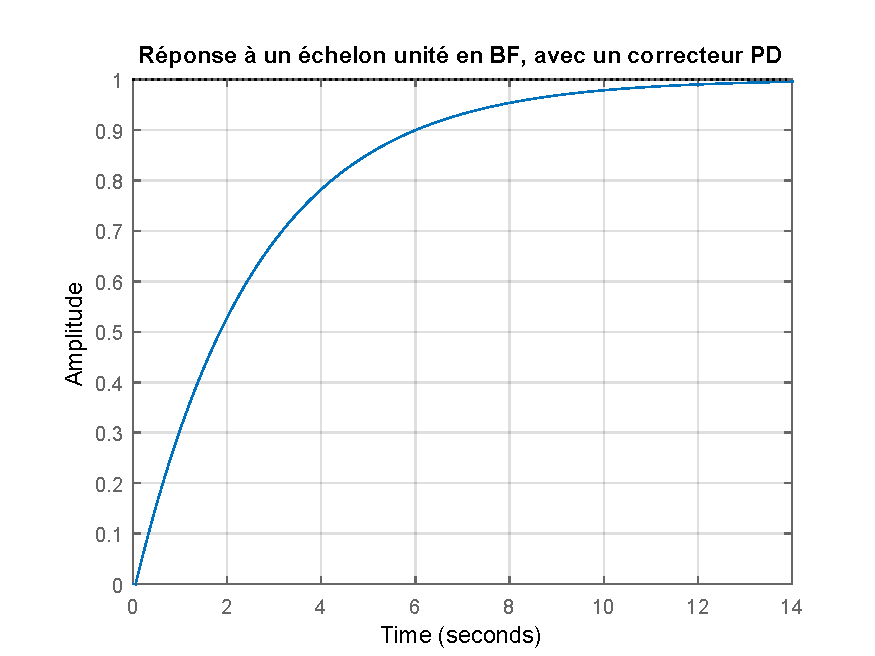
\includegraphics[width = .7\textwidth]{./II/images/rep_echelon_BF_simple.pdf}
\caption{Réponse à un échelon unité en BF, avec un correcteur PD}\label{fig:repEchelonSimple}
\end{figure}	


Nous avons réalisé une meilleure simulation, avec un fichier \emph{Simulink} danslequel nous avons relevé les signaux de sorties et d'amplitudes. Vous trouverez ces résultats aux figures \ref{fig:comEchelon} et \ref{fig:repEchelon}.
\begin{figure}[!ht]
\begin{minipage}{.5\textwidth}
\centering
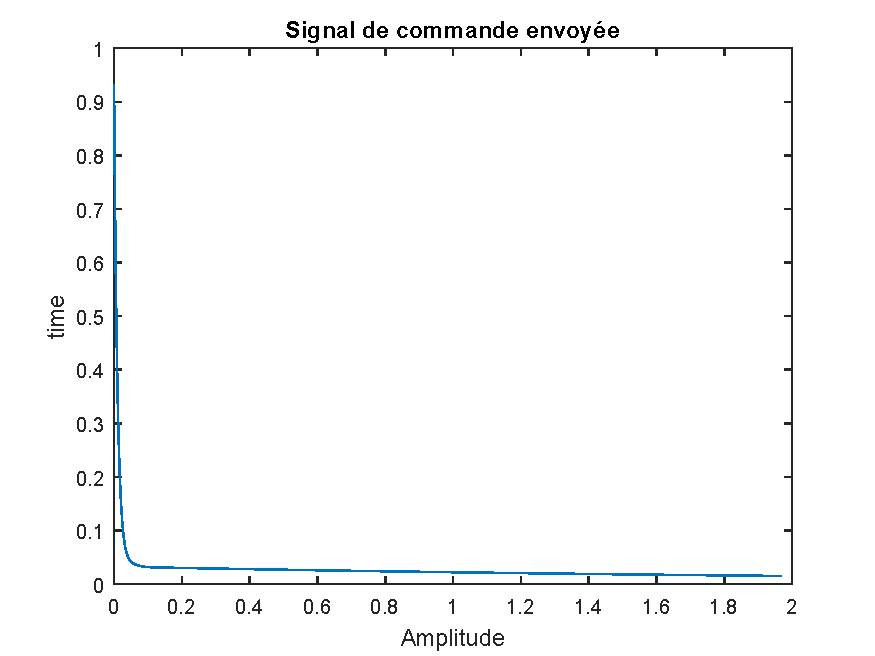
\includegraphics[width = \textwidth]{./II/images/commandePD.pdf}
\caption{Signal de commande envoyée \emph{Simulink}}\label{fig:comEchelon}
\end{minipage}
\begin{minipage}{.5\textwidth}
\centering
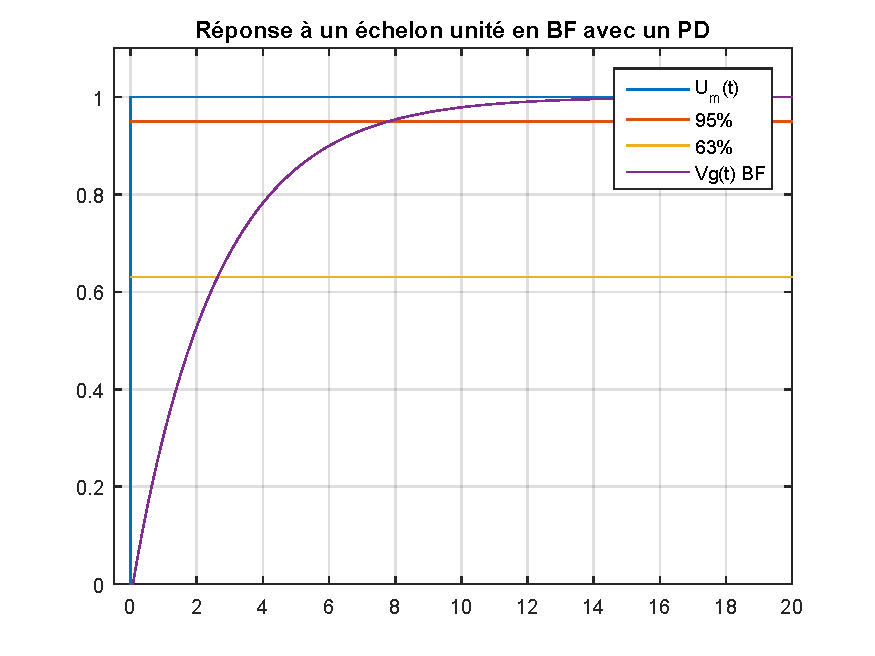
\includegraphics[width = \textwidth]{./II/images/rep_echelon_BF.pdf}
\caption{Réponse à un échelon unité en BF avec un PD \emph{Simulink}}\label{fig:repEchelon}
\end{minipage}
\end{figure}

\paragraph*{Conclusion Résultats} Nous avons bien le temps de réponse demandé dans le cahier des charges, ainsi que l'absence d'oscillations et dépassement. Le placement d'un tel correcteur nous permet de satisfaire le cahier des charges mais le retard admissibles est lui, assez faible. Nous verrons dans les parties suivantes si des correcteurs mieux adaptés aux systèmes à retards sont possibles.


\section{Équivalence avec retour d'état instantané}
Pour une loi de commande PD avec comme polynôme $Q(p) = k_1+k_2p+...+k_np^n$ dans la boucle d'asservissement, nous pouvons écrire le développement suivant : 
\begin{align*}
\frac{Y(p)}{E(p)} = \frac{G(p)}{1 + Q(p)G(p)} & \Leftrightarrow \frac{Y(p)}{E(p)} = \frac{Y(p)}{U(p) + Q(p)Y(p)}\\
&\Leftrightarrow \frac{1}{E(p)} = \frac{1}{U(p) + Q(p)Y(p)} \\
& \Leftrightarrow E(p) = U(p) + Q(p)Y(p)\\
& \Leftrightarrow U(p) = E(p) - Q(p)Y(p)
\end{align*} 
Cette dernière ligne est la caractéristique d'un retour d'état, si et seulement si les états sont disponibles sur la sortie du système.